\section{Parallel computing}

As the dimensionality of a problem increases, so often too does the time required for performing simulations. One method for accelerating numerical solutions involves the use of multiple compute cores on a central processing unit (CPU) operating independently on different data elements in unison. This form of parallel computation can be achieved through the use of the OpenMP (Open Multi-Processing) application programming interface (API), which defines how a program may parallelise certain elements of code. It allows the developer to fully utilise the power of a multicore processor. However, the limit on how much performance can be gained by this method is set by the number of compute cores available to the system, as well as the limited support offered by compilers. It should also be noted that \textsc{MATLAB} has inherent support for such programming paradigms, and fully abstracts the implementation from the developer. In this instance writing a program from scratch in C/C++/Python/etc. for such a means of parallelisation may not be very beneficial due to the cost of diminishing returns. Results would likely be obtained much faster from simply using a multicore supported package, provided one includes the time to write, as well as simulate. However, this is not always the case, given that the size of problems can often require more cores than available on a single machine.

Another widely used programming paradigm that gets around this CPU core limitation is that of MPI (message passing interface). Where OpenMP allows a user to utilise all available processing cores on a single system, MPI allows the use of an (almost) unlimited number of networked computer systems operating in parallel together, each known as a node. This is the method generally preferred in programs written for compute clusters, where a large number of nodes are available to use. It is the preferable choice for distributed computing applications, with the best performance gains given if there is minimal dependence between data. A bottleneck may occur if data spread over multiple nodes is required for an operation, requiring continual transmission of data between individual nodes. At current data rates this would be limited to bus speeds (assuming an Infiniband optical connection) on the order of tens of gigabytes per second. Compared to a local calculation requiring little to no transfers, the memory bandwidth (data quantity transferred between RAM and CPU per second) can be as high as 60 gigabytes per second \cite{DAT:Intel_xeon}. It is important to note that transfers should be minimised to avoid bottlenecks, but transfers are often necessary to make use of the large number of processing cores. Therefore, to give a significant performance benefit, a large number of cores, a high memory bandwidth, a high-speed interconnect between cores (nodes), as well as sufficient space to store the problem in memory are required. This is a tall order.

One possible means of achieving high performance is through the use of graphics processing units (GPUs). GPUs are signal processing devices, and have been highly developed over the past 20 years to offload much of the computation required to display images from the central processing unit (CPU). As a result, GPUs have been given the task of performing operations necessary to update a large number of pixels in a short amount of time, as well as complex 3D mathematics for image rendering. This has been achieved through giving the GPUs a large number of specialised compute cores for floating-point arithmetic, effectively operating in parallel. With the advent of general purpose GPU (GPGPU) computing, the ability to exploit these cores for the purpose of numerical computation has become possible. If a problem can be mapped effectively to the hardware of a GPU, it can reduce the overall compute time required for evaluating results, as well as reducing overall power usage. For the previous generation flagship industry standard GPUs used in computational acceleration (Nvidia M2090) the memory bandwidth for the device global memory (equivalent of RAM) is given as 288 gigabytes per second, with upwards of thousands of cores on demand, yielding a theoretical total of $1.41\times10^{12}$ floating-point operations per second (FLOPS), following the formula
\begin{equation}
    \text{FLOPS} = \text{cores}\times\text{clock frequency}\times\text{operations per clock cycle}.
\end{equation}

A comparison to this are Intel Xeon CPU throughput values, which at best yield approximately $10^{11}$ FLOPS. As can be seen, performance of an order of magnitude can be gained by using a GPU for calculations, over high-performance (Xeon) CPUs. This has been shown to allow for effective implementation of the previously mentioned Fourier split-operator method \cite{Num:Bauke_cpc_2011}. We have also shown that it yields performance exceeding that of CPUs for a modest choice of GPU \cite{AO:Morgan_pra_2013}, of which I will discuss in detail in a later section.

\subsection{Parallel operations}\label{subsec:par_op}
\label{sub:Parallel operations}
For a calculation to fully utilise all available throughput of a parallel-capable
compute device, it is essential to break down the problem into easily parallelised sub-problems, which can be easily achieved if data and required operations are uncoupled (\textit{embarrassingly parallel}). Considering summation as an example, imagine we have a large vector of floating point values that are to be summed together. The traditional way to solve this would be to iteratively add values to an accumulator, and return the final value at the end as the sum. This simple algorithm is $\mathcal{O}(n)$ complexity in time, as we iterate through each element at a time. Given that summation is associative, we easily parallelise this operation. By dividing our vector amongst a number of available processing cores recursively, we can reduce the computation to $\mathcal{O}(\log{} n)$ in time (see Fig.~\ref{fig:prefixsum}). This algorithm can give a significant benefit when a large number of summations are performed, such as for wavefunction normalisation, and can reduce the accumulated error resulting from floating point addition from $\mathcal{O}(n)$ to $\mathcal{O}(\log{} n)$~\cite{NUM:Higham_siam_1993}.

\begin{figure}
    \centering
    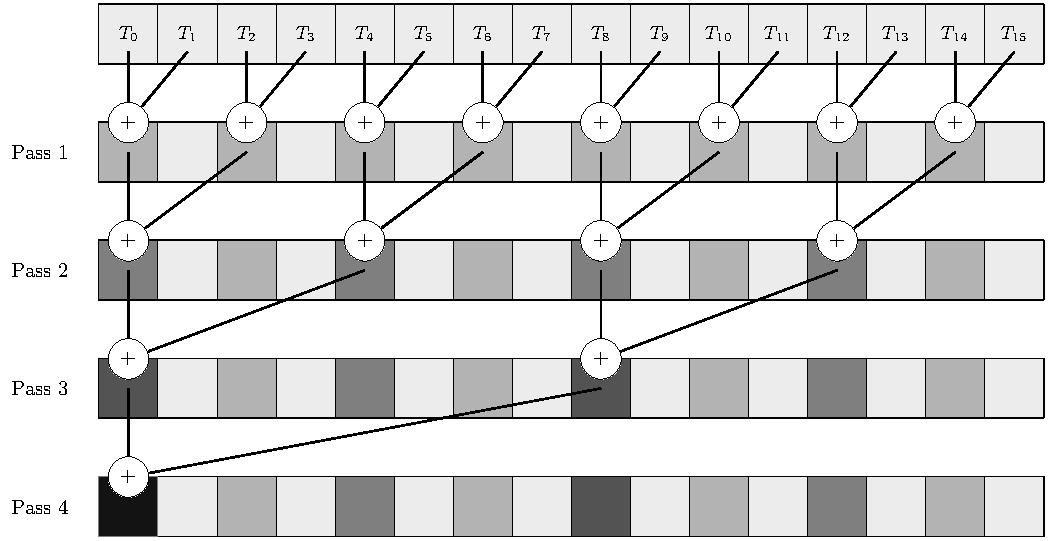
\includegraphics[width=0.75\textwidth]{./ch3_numerics/CUDA/prefixsum.pdf}
    \caption{A simplified parallel summation algorithm. After each pass the number of elements to sum is halved, leading to a $\mathcal{O}(\log{} n)$ complexity in time. Since we require only the total sum, this algorithm choses to read the value at $T_0$ at the end of the run.}
    \label{fig:prefixsum}
\end{figure}

Another typical algorithm following this is the Hadamard product (element-wise multiplication) of two vectors or matrices. Although in parallel the number of operations and complexity remains the same, the advantage comes from the lack of interdependence between elements. The multiplications can be carried out asynchronously, allowing all freely available cores to work continuously until every element pair is multiplied.


Mapping the above problems onto GPU devices requires an understanding of some of the architecture and hierarchies of the programming model. I will next introduce this model, and discuss some optimal uses of the available memory and structures.


\section{CUDA programming model}\label{sec:cuda_prog}
Although many models exist for multicore programming, for both CPU and GPU with OpenCL and OpenACC being two such examples, I will concentrate on Nvidia's CUDA \cite{NUM:Nickolls_cuda_2008}. CUDA is a mature programming model and API for Nvidia GPUs, and has been well-received for high-performance parallel computing. CUDA operates on a single instruction multiple thread (SIMT) architecture, wherein a single operation is mapped to multiple compute threads independently operating on individual units of data. Writing a program using CUDA C/C++ is very similar to standard C/C++ programming, albeit with some minor differences to account for control of GPU compute threads. CUDA manages calculations in a hierarchical structure with differing levels of fine-grained control over these threads. At the finest grained level ($T$) we have compute threads which operate directly on a single datum from memory. The maximum number of threads which can run simultaneously on the device in a single compute unit are known as a \textit{warp}. Threads are grouped into blocks ($\mathbf{B}$), which is the next hierarchical level, which will optimally contain multiples of the maximum warp number for the device (32 elements is the standard warp size for Nvidia architecture).

At the coarsest level, the blocks are grouped together into a grid ($\mathbf{G}$), which encompasses the entire problem space. Hardware limits are specified limiting the upper-values of how many elements can appear in these units, and thus the hierarchy exists to allow for fine-grained control on memory usage, and hence performance optimisation on calculations. For a given problem it is necessary to find a mapping from data values in memory to execution threads. To ensure optimal use of GPU cores, the number of threads worked on simultaneously can be (for current hardware) up to 1024 threads per block, though keeping this value divisible by the warp size is recommended to allow exact mapping to device cores. Optimal values can be found for balancing data computation and transfers, giving, depending on system size, necessary values for block size, as well as grid size. The dimensions of each hierarchical layer are independent of one another, and may be up to 3, with a hardware dependent limit only imposed on the maximum number of elements. Figure~\ref{fig:gpu_threads} gives a sample layout for a system of 2D threads, 2D blocks, and a single grid.

\begin{figure}[tb]
    \centering
    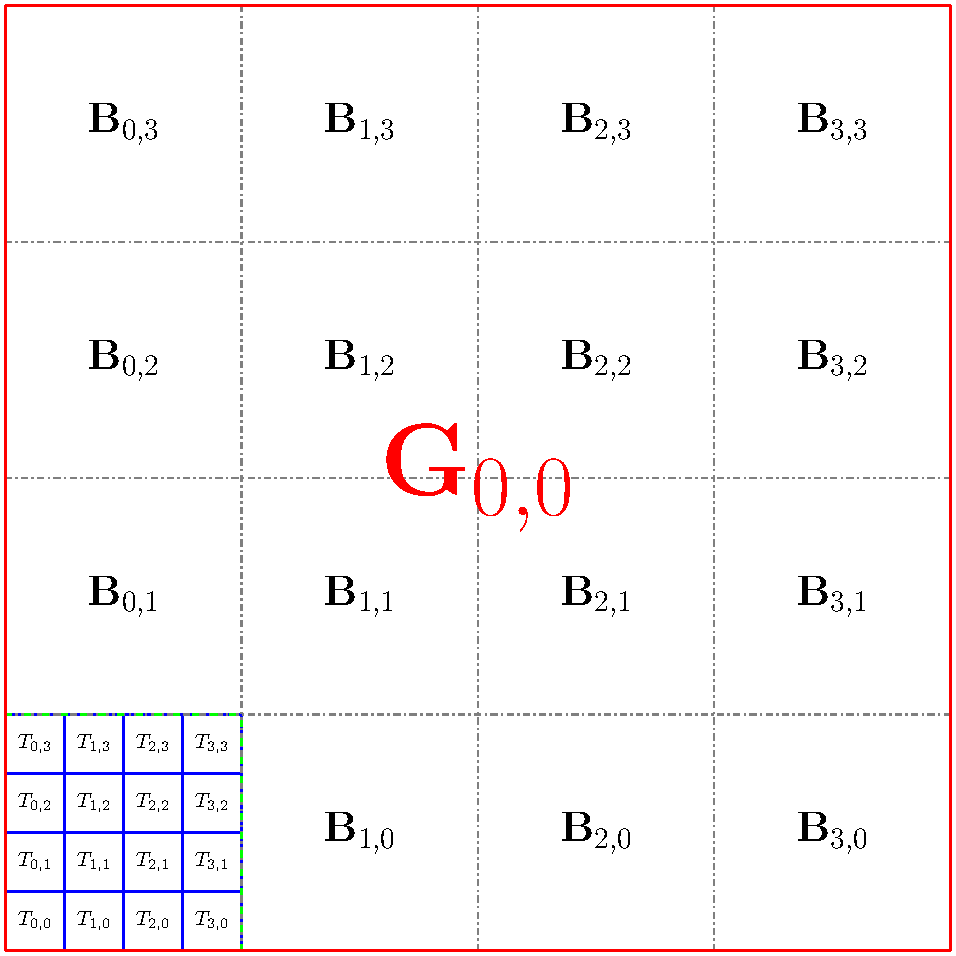
\includegraphics[width=0.6\textwidth]{./ch3_numerics/CUDA/gputhreads.pdf}
    \caption{A sample CUDA data hierarchy model. Each thread ($T_{x,y}$) has use of private memory, which offers the highest performance overall, though does not allow transfer to other threads. Data within a block ($\mathbf{B_{x,y}}$)can be treated as adjacent and accessible to all other elements in the block using {shared memory}, and is next highest in terms of performance. Transfers between blocks require the use of {global memory}, which is slowest overall. Internally all data is stored and indexed lexicographically within the grid ($\mathbf{G}_{x,y}$).}
    \label{fig:gpu_threads}
\end{figure}

It is necessary to be aware of the different aspects of managing the GPU memory. Unlike programming for a CPU-based system, GPUs require explicit control of several different types of memory. Nvidia's CUDA programming model defines these different physical memories into \textit{global}, \textit{constant}, \textit{shared} and \textit{private}. Global memory is analogous to random access memory (RAM) on a CPU-based system, and is the location where we primarily store data for computation on the GPU. This memory block is accessible (readable and writeable) to all threads in the computation. This is also the slowest memory on the GPU, with bandwidths of approximately $10^{11}$ bytes per second. Constantly reading and writing to global memory can hinder the performance of a computation. For memory that is statically defined at the start of a program and will only be read thereafter, the constant memory can be used. This is a special area of memory that can be used to store constants and other values that are often read during a computation. Once set, these values cannot be modified. The next memory level is shared memory, which is block accessible only i.e. threads within the same block have access. This allows threads to exchange information with close neighbours, and is the preferred method of inter-thread communication. Although higher performance than global, the size of shared memory is much smaller. An ideal use case is the parallel summation example given in Sec.~\ref{subsec:par_op}. Performing this algorithm requires the copying of data from global to shared memory, performing the calculations, then copying the results back. Lastly, private memory which maps directly to device cache, is thread-accessible only i.e. each thread has access only to its own private values. This memory can be used for local variables defined in a function (known as a \textit{kernel} for GPUs). Private memory has the highest performance, but the smallest available size. If possible, copying variables from global memory into private memory, performing all operations on private, then saving back to global can yield the highest performance, as global memory (slow) is read from and written to once each.

Limiting transfers between the CPU/RAM to the GPU/global memory are of high importance, as the slowest line of communication is the PCI-Express bus, connecting the GPU to the host system ($\approx 16 $ GB/s max). Eliminating unnecessary communication will almost certainly allow for a gain in performance. Mapping a problem to the GPU requires parallelising the calculation and removing transfers where applicable. For maximum performance, a sample model of performing a GPU calculation is:
\begin{enumerate}
    \item Define all variables and data on the host system.
    \item Identify the optimal mapping onto the GPU thread execution model.
    \item Send the data from RAM to the GPU global memory.
    \item Perform computation, with necessary elements copied to shared/private memory.
    \item Return final output of computation to host system when completed.
\end{enumerate}

Although idealised and highly simplified, close adherence to such a model should yield significant performance gains compared to multicore CPU-based computation. An important point with memory access in GPUs is that to ensure optimal performance all access should be assumed to be in-order and adjacent. As an example, though the parallel sum method discussed in Sec.~\ref{subsec:par_op} is superior to an iterative summation, it is not an optimal example for GPU architectures \cite{BK:Cuda_book}. With a small improvement, this can be highly optimised, as highlighted by Fig.~\ref{fig:prefixsum2}. In this case, the memory access is carried out in strided linear chunks, and by ensuring that all memory accesses are performed this way as much as possible an overall higher degree of performance can be achieved \cite{BK:Cuda_book}. As GPUs operate on blocks of memory simultaneously, minimising the amount of misaligned memory accesses can optimise the access performance. In this instance, these structures can be packed efficiently together and ensure a large number of copies are performed optimally, with coalesced memory access.

While the details are often abstracted by the internal workings of the device, an awareness of this can prove useful. If we assume the number of data elements to be summed is larger than the available number of threads, this routine can perform several passes before the threads become sub-optimally used, as in the previous case. In this way, the summation ensures that the available threads are working mostly optimally.

\begin{figure}
    \centering
    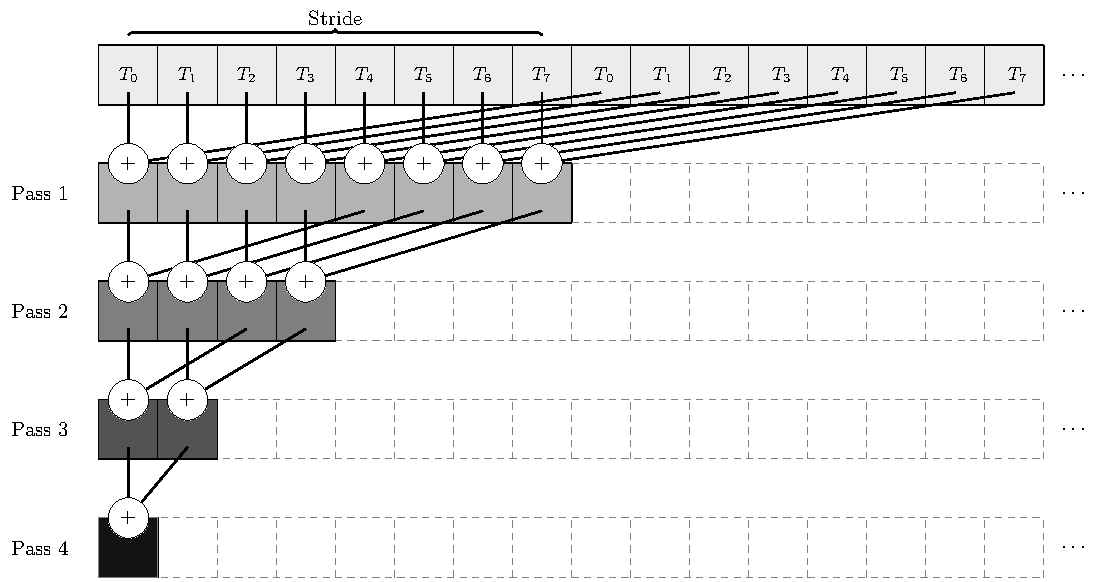
\includegraphics[width=0.75\textwidth]{./ch3_numerics/CUDA/prefixsum_2.pdf}
    \caption{An optimised parallel summation, which allows for strided memory access. By halving the size of the stride and block size at every increment the number of evaluations carried out simultaneously will better utilise the available GPU cores.}
    \label{fig:prefixsum2}
\end{figure}

Given that GPUs are first and foremost image processing devices, their ability to perform Fourier transforms rapidly is a well developed strength. Due to the large number of available cores, fast Fourier transforms (FFTs) can be significantly faster on a GPU than performing the same operation on many CPUs \cite{AO:Morgan_pra_2013}. The CUFFT library allows for a seamless way to take advantage of this performance increase using GPUs. Next, I will discuss an example of GPU-enabled simulations for an experimentally realistic problem making use of the GPU to perform the necessary operations discussed in Sec.~\ref{sec:timeev},\ref{sec:fso}, and offer some realistic performance measurements.

%\section{3D STIRAP using GPU}
%For performance metrics, I will discuss the use of a GPU-enabled Schr\"odinger equation integrator developed by myself, comparing the results to a multi-core MPI enabled version by T. Morgan and N. Crowley. We solved the Schr\"odinger equation for a fully three-dimensional potential, demonstrating its accuracy and improved performance compared to standard HPC methods.
